% 115-83(115쪽) — 정사각형에서 각 변의 중점을 이어 정사각형을 그리는 시행을 반복해 그린 T_1, T_2, T_3.
% 스캔 화질이 낮아 TikZ 로 다시 그림. 라벨은 원문 그대로 T_1·T_2·T_3 만 두고 한 변의 길이(답)는 적지 않는다.
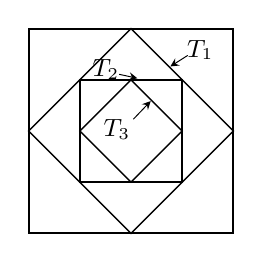
\begin{tikzpicture}[line width=0.5pt]
  \draw[line width=0.7pt] (0,0) rectangle (2.6,2.6);
  \draw (1.3,0) -- (2.6,1.3) -- (1.3,2.6) -- (0,1.3) -- cycle;
  \draw (0.65,0.65) rectangle (1.95,1.95);
  \draw (1.3,0.65) -- (1.95,1.3) -- (1.3,1.95) -- (0.65,1.3) -- cycle;
  \draw[->, >=stealth, line width=0.35pt] (1.15,2.02) -- (1.38,1.97);
  \node[font=\small] at (0.98,2.08) {$T_2$};
  \draw[->, >=stealth, line width=0.35pt] (2.02,2.26) -- (1.80,2.12);
  \node[font=\small] at (2.18,2.33) {$T_1$};
  \draw[->, >=stealth, line width=0.35pt] (1.33,1.45) -- (1.55,1.68);
  \node[font=\small] at (1.12,1.32) {$T_3$};
\end{tikzpicture}
